\chapter{Metodologia}
\label{chap:metodologia}

%\lipsum[2]
%
%\begin{figure}[h!]
%	\caption{Mapa conceitual do estudo da história e relações com o objeto de estudo}
%	\label{fig_mapa}
%	\begin{center}
%		\fbox{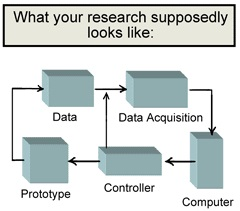
\includegraphics[width=8cm]{figuras/figura-1}}
%	\end{center}
%	\fontedafigura{8cm}{os autores}
%\end{figure}
%
%\lipsum[2]

O Gráfico 1 apresenta a distribuição anual da produção, realizando-se uma comparação entre a produção de dissertações de mestrado e teses de doutorado.

\begin{figure}[h!]
	\centering
	\caption{Produção anual das dissertações de mestrado e teses de doutorado entre os anos de 1990 e 2008}
	\label{fig_mapa}
	\fbox{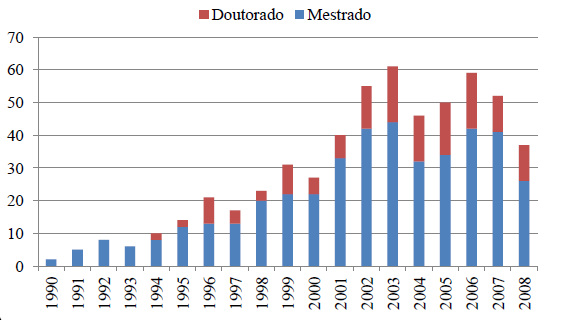
\includegraphics{figuras/figura-3}}
	\fontedafigura{os autores}{os autores}
\end{figure}

Nota-se a partir do Gráfico 1 e da Tabela 1 que a produção de teses de doutorado teve seu início no ano de 1994, esta informação se justifica devido ao fato de que os cursos de doutorado na área da Saúde Coletiva começaram a surgir no país a partir do ano de 1990, que coincide com o ano de implantação do SUS. As duas primeiras teses com o ano de 1994 fazem parte do doutorado em Saúde Coletiva da UNICAMP e do Doutorado em saúde Pública da USP. Nos anos de 2003 e 2006, houve uma produção mais elevada no que diz respeito às teses de doutorado, se comparada com a produção dos outros anos. Observa-se também que 2003 e 2006 são os anos de maior pico de produção científica de temas relacionados ao campo do trabalho.